\documentclass[a4paper,11pt]{exam}
\printanswers % pour imprimer les réponses (corrigé)
%\noprintanswers % Pour ne pas imprimer les réponses (énoncé)
\addpoints % Pour compter les points
% \noaddpoints % pour ne pas compter les points
%\qformat{\textbf{\thequestion )}}
%\qformat{\textbf{\thequestion )} (\thepoints) \\ } % Pour définir le style des questions (facultatif)
\usepackage{color} % définit une nouvelle couleur
\shadedsolutions % définit le style des réponses
% \framedsolutions % définit le style des réponses
\definecolor{SolutionColor}{rgb}{0.8,0.9,1} % bleu ciel
\renewcommand{\solutiontitle}{\noindent\textbf{Solution:}\par\noindent} % Définit le titre des solutions




\makeatletter

\def\maketitle{{\centering%
	\par{\huge\textbf{\@title}}%
	\par{\@date}%
	\par}}

\makeatother

\lhead{NOM Pr\'enom :}
\rhead{\textbf{Les r\'eponses doivent \^etre justifi\'ees}}
\cfoot{\thepage / \pageref{LastPage}}


%\usepackage{../../pas-math}
%\usepackage{../../moncours}


%\usepackage{pas-cours}
%-------------------------------------------------------------------------------
%          -Packages nécessaires pour écrire en Français et en UTF8-
%-------------------------------------------------------------------------------
\usepackage[utf8]{inputenc}
\usepackage[frenchb]{babel}
\usepackage[T1]{fontenc}
\usepackage{lmodern}
\usepackage{textcomp}



%-------------------------------------------------------------------------------

%-------------------------------------------------------------------------------
%                          -Outils de mise en forme-
%-------------------------------------------------------------------------------
\usepackage{hyperref}
\hypersetup{pdfstartview=XYZ}
%\usepackage{enumerate}
\usepackage{graphicx}
\usepackage{multicol}
\usepackage{tabularx}
\usepackage{multirow}


\usepackage{anysize} %%pour pouvoir mettre les marges qu'on veut
%\marginsize{2.5cm}{2.5cm}{2.5cm}{2.5cm}

\usepackage{indentfirst} %%pour que les premier paragraphes soient aussi indentés
\usepackage{verbatim}
\usepackage{enumitem}
\usepackage[usenames,dvipsnames,svgnames,table]{xcolor}

\usepackage{variations}

%-------------------------------------------------------------------------------


%-------------------------------------------------------------------------------
%                  -Nécessaires pour écrire des mathématiques-
%-------------------------------------------------------------------------------
\usepackage{amsfonts}
\usepackage{amssymb}
\usepackage{amsmath}
\usepackage{amsthm}
\usepackage{tikz}
\usepackage{xlop}
%-------------------------------------------------------------------------------



%-------------------------------------------------------------------------------


%-------------------------------------------------------------------------------
%                    - Mise en forme avancée
%-------------------------------------------------------------------------------

\usepackage{ifthen}
\usepackage{ifmtarg}


\newcommand{\ifTrue}[2]{\ifthenelse{\equal{#1}{true}}{#2}{$\qquad \qquad$}}

%-------------------------------------------------------------------------------

%-------------------------------------------------------------------------------
%                     -Mise en forme d'exercices-
%-------------------------------------------------------------------------------
%\newtheoremstyle{exostyle}
%{\topsep}% espace avant
%{\topsep}% espace apres
%{}% Police utilisee par le style de thm
%{}% Indentation (vide = aucune, \parindent = indentation paragraphe)
%{\bfseries}% Police du titre de thm
%{.}% Signe de ponctuation apres le titre du thm
%{ }% Espace apres le titre du thm (\newline = linebreak)
%{\thmname{#1}\thmnumber{ #2}\thmnote{. \normalfont{\textit{#3}}}}% composants du titre du thm : \thmname = nom du thm, \thmnumber = numéro du thm, \thmnote = sous-titre du thm

%\theoremstyle{exostyle}
%\newtheorem{exercice}{Exercice}
%
%\newenvironment{questions}{
%\begin{enumerate}[\hspace{12pt}\bfseries\itshape a.]}{\end{enumerate}
%} %mettre un 1 à la place du a si on veut des numéros au lieu de lettres pour les questions 
%-------------------------------------------------------------------------------

%-------------------------------------------------------------------------------
%                    - Mise en forme de tableaux -
%-------------------------------------------------------------------------------

\renewcommand{\arraystretch}{1.7}

\setlength{\tabcolsep}{1.2cm}

%-------------------------------------------------------------------------------



%-------------------------------------------------------------------------------
%                    - Racourcis d'écriture -
%-------------------------------------------------------------------------------

% Angles orientés (couples de vecteurs)
\newcommand{\aopp}[2]{(\vec{#1}, \vec{#2})} %Les deuc vecteurs sont positifs
\newcommand{\aopn}[2]{(\vec{#1}, -\vec{#2})} %Le second vecteur est négatif
\newcommand{\aonp}[2]{(-\vec{#1}, \vec{#2})} %Le premier vecteur est négatif
\newcommand{\aonn}[2]{(-\vec{#1}, -\vec{#2})} %Les deux vecteurs sont négatifs

%Ensembles mathématiques
\newcommand{\naturels}{\mathbb{N}} %Nombres naturels
\newcommand{\relatifs}{\mathbb{Z}} %Nombres relatifs
\newcommand{\rationnels}{\mathbb{Q}} %Nombres rationnels
\newcommand{\reels}{\mathbb{R}} %Nombres réels
\newcommand{\complexes}{\mathbb{C}} %Nombres complexes


%Intégration des parenthèses aux cosinus
\newcommand{\cosP}[1]{\cos\left(#1\right)}
\newcommand{\sinP}[1]{\sin\left(#1\right)}


%Probas stats
\newcommand{\stat}{statistique}
\newcommand{\stats}{statistiques}
%-------------------------------------------------------------------------------

%-------------------------------------------------------------------------------
%                    - Mise en page -
%-------------------------------------------------------------------------------

\newcommand{\twoCol}[1]{\begin{multicols}{2}#1\end{multicols}}


\setenumerate[1]{font=\bfseries,label=\textit{\alph*})}
\setenumerate[2]{font=\bfseries,label=\arabic*)}


%-------------------------------------------------------------------------------
%                    - Elements cours -
%-------------------------------------------------------------------------------





%\usepackage{fullpage}
\author{\ }
\date{13 Janvier 2021}
\title{$6^e 2$ : DS num\'ero 3}


\begin{document}
%	\usepackage{fancyhdr}
%	
%	\pagestyle{fancy}
%	\fancyhf{}
	%\rhead{Share\LaTeX}

	\maketitle
	
%\begin{center}
%	\textbf{Aucun des exercices n'est à faire sur cette feuille}
%\end{center}

\begin{small}
	\begin{center}
		\begin{tabular}{|@{\ }l@{\ }|@{\ }c@{\ }|@{\ }c@{\ }|@{\ }c@{\ }|@{\ }c@{\ }|}
			\hline
			\textbf{Compétence} & \textbf{MI} & \textbf{MF} & \textbf{MS} & \textbf{TBM} \\
			\hline
			\textbf{Calculer} (Mon résultat semble correct) &  \ \ & \ \ & \ \ & \ \  \\
			\hline
			\textbf{Calculer} (Je calcule des sommes, différences ou produits de nombres décimaux)&  \ \ & \ \ & \ \ & \ \  \\
			\hline
			\textbf{Calculer} (Je respecte les priorités opératoires)&  \ \ & \ \ & \ \ & \ \  \\
			\hline	
			\textbf{Raisonner} (Je résous des problèmes) & \ \ & \ \ &  \ \  & \ \ \\
			\hline
%			 
%			\hline
		\end{tabular}
	\end{center}
\end{small}	

	
	
%\section{Home Cinema (4 points)}

Sur un catalogue, un ensemble \textit{Home Cinema} est vendu \num{2088.64} €.
Si on choisi de payer par mensualités, on règle \num{205.22} € à la commande et \num{175.95} € par mois pendant 11 mois.

\begin{questions}
	\question[2] Combien va-t-on payer si on choisit le paiement par mensualités ?
	\begin{solution}
		\begin{equation*}
			\num{205.22} + 11 \times \num{175.95} = \num{2140.67}
		\end{equation*}
		
		Avec paiement par mensualités on paiera au final \num{2140.67} euros.
	\end{solution}
	
	\question[2] En payant en une seule fois, combien aurait-on économisé ?
	\begin{solution}
		\begin{equation*}
		\num{2140.67} - \num{2088.64} = \num{52.03}
		\end{equation*}
		
		Un paiement en une seule fois ferait économiser \num{52.03} euros.
	\end{solution}
		
\end{questions}	

\section{Calcul}

Calculer en détaillant les calculs :

\begin{questions}
	\question $A = (+7) - (-5) + (-11) - (-4) + (-7)$
	
	\question $B = (+13) + (-5) - (+14) - (+17) - (-13)$
	
	\question $C = (\num{-2.8}) - (\num{+3.7}) - (\num{+4.1}) + (\num{-2.3}) - (\num{+4.5})$
	
	\question $D = (\num{-8.1}) - (\num{+3.6}) + (\num{-9.7}) - (\num{-8.2}) - (\num{-2.4})$
	
	\question $E = \num{2.5} - \num{3.9} + \num{4.9} - \num{1.5} - 3$
	
	\question $F = \num{12.3} - \num{32.1} + \num{21.3} - \num{13.2}$
\end{questions} 

\section{Conversions (\`A faire sur cette feuille) }


\begin{center}
	\begin{tabular}{|@{\ \ \ }c@{\ \ \ }|@{\ \ \ }c@{\ \ \ }|@{\ \ \ }c@{\ \ \ }|@{\ \ \ }c@{\ \ \ }|@{\ \ \ }c@{\ \ \ }|@{\ \ \ }c@{\ \ \ }|@{\ \ \ }c@{\ \ \ }|}
		\hline
		\ \ \ \ \ \ \ \  & \textbf{hm} & \textbf{dam} & \ \ \ \ \ \ \ \    & \ \ \ \ \ \ \ \   & \ \ \ \ \ \ \ \  & \textbf{mm} \\ \hline
		&             & 1            & 2 &  &  &             \\ \hline
		&             &              &   &  &  &             \\ \hline
		&             &              &   &  &  &             \\ \hline
		&             &              &   &  &  &             \\ \hline
	\end{tabular}
\end{center}

\begin{questions}
	\question Compléter la première ligne du tableau de conversion (le nom des colonnes).
	
	\question A l'aide du tableau, compléter :
		\begin{parts}
			\begin{multicols}{2}
				\part  $12 \ m = \hspace*{3cm} cm$.
				\part $15 \ dm = \hspace*{3cm} hm$.
				\part $145 \ dam = \hspace*{3cm} mm$.
				\part $\num{18.5} \ hm = \hspace*{3cm} m$.	
			\end{multicols}
			 
		\end{parts}
\end{questions}

\newpage

\section{Ordres de grandeur (4 points)}

Déterminer un ordre de grandeur le plus précis possible de :

\begin{questions}
	\question[1] $\num{30.02} \times \num{12.3} + 98$
	\begin{solution}
		$\num{30}	\times 10 + 100 = 400	$
		Le résultat est proche de 400.
	\end{solution}
	\question[1] $\num{203.58} + \num{502.2} \times \num{3.9}$
	\begin{solution}
		$\num{200}	+ 500 \times 4 = 2200	$
		Le résultat est proche de 2200.
	\end{solution}
	\question[1] $(\num{54.123} + \num{48.9}) \times \num{0.9}$
	\begin{solution}
		$\num{50}	+ 50 \times 1 = 100	$
		Le résultat est proche de 100.
	\end{solution}

	\question[1] $\num{794.9} \times \num{1.2} \times \num{19.875}$
	\begin{solution}
		$\num{1000}	\times 1 \times 20 = \num{20000}	$
		Le résultat est proche de \num{20000}.
	\end{solution}
\end{questions}
%\section{Porte conteneurs (3 points)}

Un porte-conteneur transporte des conteneurs identiques et de même masse.
Lorsqu'il quitte le port de Hanovre, sa masse est de \num{61750} tonnes.
Au port du Havre, il débarque la moitié de ses conteneurs. Le bateau ne pèse plus que \num{50875} tonnes.

\begin{questions}
	\question[1] Quelle est la masse des conteneurs débarqués ?
	\begin{solution}
		\begin{equation*}
			\num{61750} - \num{50875} = \num{10875}
		\end{equation*}
		
		La masse des des conteneurs débarqués est \num{10875} tonnes.
	\end{solution}

	\question[1] Quelle est la masse du porte-conteneur à vide ?
	
	\begin{solution}
		Les conteneurs débarqués au havre représente la moitié de son chargement, il reste donc une masse équivalente.
		
		\begin{equation*}
			\num{50875} - \num{10875} = \num{40000}
		\end{equation*}
		
		Donc la masse du porte-conteneur à vide est \num{40000} tonnes.
	\end{solution}

	\question[1] Convertir  \num{10875} tonnes en kilogrammes ?
\end{questions}

%\section{Vocabulaire (4 points)}

\begin{questions}
	\question[2] \'Ecrire le nombre 15 comme une somme de deux produits.
	\begin{solution}
		\begin{equation*}
			5 \times 2 + 5 \times 1 = 15
		\end{equation*}
	\end{solution}
	
	\question[2] \'Ecrire le nombre 15 comme un produit de deux sommes.
	
	\begin{solution}
		\begin{equation*}
		(1 + 2) \times (3 + 2) = 15
		\end{equation*}
	\end{solution}
	
\end{questions}


\section{Calcul d'expressions}

\begin{questions}
	\question Calculer les expressions suivantes en détaillant toutes les étapes du calcul.
	\begin{multicols}{2}
		\begin{parts}
			\part $A = \num{7.25} + \num{6.1} + \num{5.75} + \num{3.9}$
			\begin{solution}
				\begin{eqnarray*}
					A &=& \num{7.25} + \num{6.1} + \num{5.75} + \num{3.9} \\
					A &=& \num{7.25} + \num{5.75} + \num{6.1} + \num{3.9} \\
					A &=& 13 + 10 \\
					A &=& 23 
				\end{eqnarray*}
			\end{solution}
			
			\part $B = 25 + 5 \times 8$
			\begin{solution}
				\begin{eqnarray*}
					B &=& 25 + 5 \times 8 \\
					B &=& 25 + 40 \\
					B &=& 65 \\
				\end{eqnarray*}
			
				\vspace*{0.5cm}
			\end{solution}
		
			\part $C = 4 + 6 \times 3 + \num{6.25} \times 4$
			\begin{solution}
				\begin{eqnarray*}
					C &=& 4 + 6 \times 3 + \num{6.25} \times 4 \\
					C &=& 4 + 18 + 25 \\
					C &=& 22 + 25 \\
					C &=& 47 
				\end{eqnarray*}
			\end{solution}
		
			\part $D = \num{3.5} \times (9 + \num{4.5} + \num{2.3}$
			\begin{solution}
				\begin{eqnarray*}
					D &=& \num{3.5} \times (9 + \num{4.5} + \num{2.3}) \\
					D &=& \num{3.5} \times (9 + \num{6.8}) \\
					D &=& \num{3.5} \times  \num{15.8} \\
					D &=& \num{55.3} 
				\end{eqnarray*}
			\end{solution}
		\end{parts}
	\end{multicols}	
	

	\question Rajouter des parenthèse (uniquement celles qui sont indispensables) pour que les égalités soient correctes. Vérifier en détaillant le calcul.
	
	\begin{parts}
		\begin{multicols}{2}
			\part $1 + 4 \times 6 = 30$
			\begin{solution}
				\begin{eqnarray*}
					(1 + 4) \times 6 &=& 5 \times 6 \\
					(1 + 4) \times 6 &=& 30 
				\end{eqnarray*}
			\end{solution}
			
			\part $34 - 12 + 22 = 0$
			\begin{solution}
				\begin{eqnarray*}
					34 - (12 + 22) &=& 34 - 34 \\
					34 - (12 + 22) &=& 0 
				\end{eqnarray*}
			\end{solution}
		
			\part $17 - 4 \times 4 = 2 \times 17 + 9$
			\begin{solution}
				\begin{eqnarray*}
					(17 - 4) \times 4 &=& 13 \times 4 \\
					(17 - 4) \times 4  &=& 52 
				\end{eqnarray*}
			
				\begin{eqnarray*}
					2 \times (17 + 9) &=& 2 \times 26 \\
					2 \times (17 + 9)  &=& 53 
				\end{eqnarray*}
			\end{solution}
		
			\part $4 + 5 \times 6 + 3 = 81$
			\begin{solution}
				\begin{eqnarray*}
					(4 + 5) \times (6 + 3) &=& 9 \times 9 \\
					(4 + 5) \times (6 + 3) &=& 81 
				\end{eqnarray*}
			\end{solution}	
		\end{multicols}
		
	\end{parts}
\end{questions}
%\section{Calculs (5 points)}

\begin{questions}


\question Compléter ce tableau (le détail des calculs n'est pas demandé) :

\begin{center}
	{\Large \begin{tabular}{|@{\ }c@{\ }|@{\ }c@{\ }|@{\ }c@{\ }|@{\ }c@{\ }|@{\ }c@{\ }|@{\ }c@{\ }|}
	\hline
	\textbf{a} & \textbf{b} & \textbf{c} & \textbf{$a-b \times c$} & \textbf{$(a-b) \times c$} & \textbf{$a + b - c$} \\ \hline
	12         & 3          & 4          &                         &                           &                      \\ \hline
	48         & 8          & 6          &                         &                           &                      \\ \hline
	\num{7.5}  & \num{2.5}  & 2          &                         &                           &                      \\ \hline
	8          & 3          & \num{1.5}  &                         &                           &                      \\ \hline
	\num{7.7}  & \num{3.9}  & 0          &                         &                           &                      \\ \hline
\end{tabular}}
\end{center}


\begin{solution}
	\begin{center}
		{\Large \begin{tabular}{|@{\ }c@{\ }|@{\ }c@{\ }|@{\ }c@{\ }|@{\ }c@{\ }|@{\ }c@{\ }|@{\ }c@{\ }|}
				\hline
				\textbf{a} & \textbf{b} & \textbf{c} & \textbf{$a-b \times c$} & \textbf{$(a-b) \times c$} & \textbf{$a + b - c$} \\ \hline
				12         & 3          & 4          & 0                       &   36                      &   11                 \\ \hline
				48         & 8          & 6          & 0                       &   240                     &       50             \\ \hline
				\num{7.5}  & \num{2.5}  & 2          &  \num{2.5}              &   10                      &        8             \\ \hline
				8          & 3          & \num{1.5}  &  \num{3.5}              &  \num{7.5}                &   \num{9.5}          \\ \hline
				\num{7.7}  & \num{3.9}  & 0          &  \num{7.7}              & 0                         &  \num{11.6}          \\ \hline
		\end{tabular}}
	\end{center}
\end{solution}
\end{questions}

%
\section{Au supermarché}

Joshua achète \num{3.4} kg de poires à \num{1,70} € le kilogramme, un fromage à \num{2.35} € l'unité et un rôti.
Il paie avec 3 billets de 10 €. La caissière lui rend \num{5.25} €.

\begin{questions}
	\question Quel calcul sur une ligne permet de connaître le prix du rôti ?
	\begin{solution}
		Calcul du prix des poires :
		
		\opmul[style=text]{3.4}{1.70}
		
		Il paye \num{5.78} € pour les poires.\\
		
		Calcul du prix payé :
		
		\opmul[style=text]{30}{3}
		
		Il paye 30 €.\\
		
		Calcul du prix des courses :
		\opsub[style=text]{30}{5.25}
		
		Le prix des courses s'élève à \num{24.75} €.\\
		
		L'expression permettant de calculer le prix du rôti est
		
		\begin{equation}
			(10 \times 3 - \num{5.25}) - (\num{3.4} \times \num{1.70} + \num{2.35})
		\end{equation}
		
	\end{solution}
	\question Quel est le prix du rôti ?
	\begin{solution}
		Calcul du prix du rôti :
		
		
		\begin{eqnarray*}
			A &=& (10 \times 3 - \num{5.25}) - (\num{3.4} \times \num{1.70} + \num{2.35}) \\
			A &=& (30 - \num{5.25}) - (\num{5.78} + \num{2.35}) \\
			A &=& \num{24.75} - \num{8.13} \\
			A &=& \num{16.62}
		\end{eqnarray*}
	
		Le rôti coûte \num{16.62} €.
	\end{solution}
\end{questions}

\newpage
\section{Bonus : Envoi d'un courrier (3 points)}

Le tableau ci-dessous présente des tarifs d'envoi de courrier de la Poste (en 2009) :

\begin{center}
	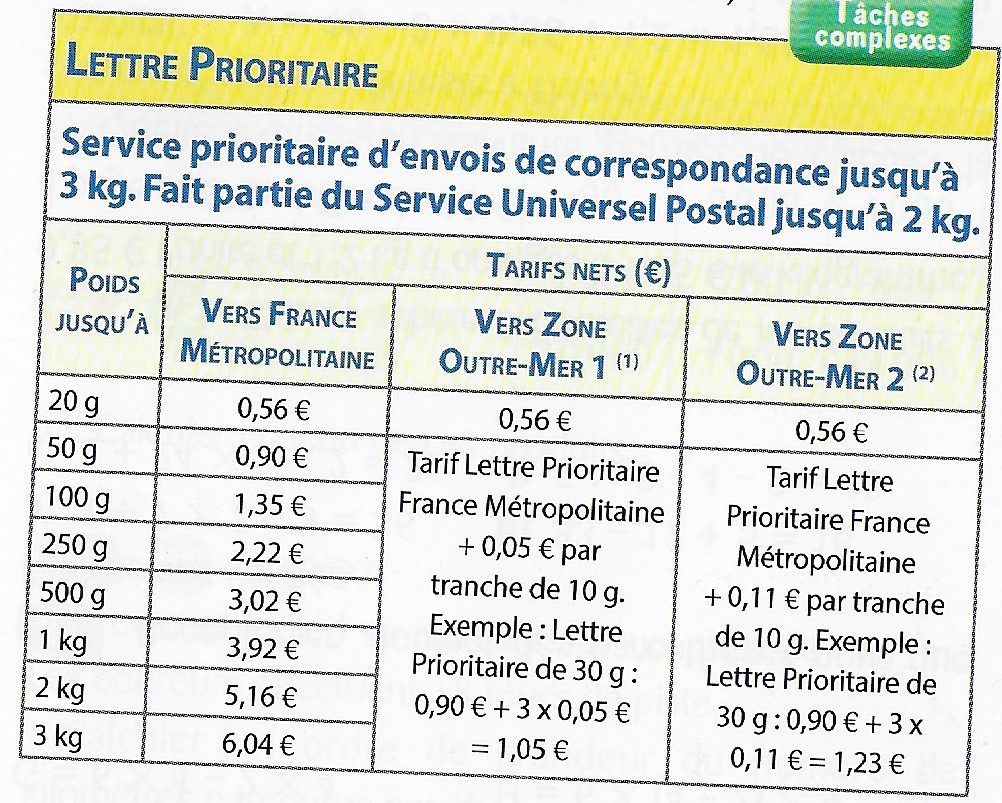
\includegraphics[scale=1.1]{img/poste}
\end{center}

\begin{questions}
	\question[1] Virginie envoie une lettre de 180 g vers la \textbf{Zone Outre-Mer 1}. Vérifier qu'elle va payer \num{3.12} €
	
	\question[1] Cathy envoie une lettre de 2 kg vers la \textbf{Zone Outre-Mer 2}. Combien va-t-elle payer ?
	
	\question[1] Théo poste une lettre pour la \textbf{Zone Outre-Mer 2}, il paye \num{6.32} €. Quelle est la masse maximale de sa lettre ?
	

\end{questions}




\label{LastPage}

%\section{Consommation électrique}
%
%Une consommation d'électricité se mesure en 
\end{document}